\documentclass[11pt, oneside]{article}   	% use "amsart" instead of "article" for AMSLaTeX format
\usepackage{geometry}                		% See geometry.pdf to learn the layout options. There are lots.
\geometry{letterpaper}                   		% ... or a4paper or a5paper or ... 
%\geometry{landscape}                		% Activate for rotated page geometry
%\usepackage[parfill]{parskip}    		% Activate to begin paragraphs with an empty line rather than an indent
\usepackage{graphicx}				% Use pdf, png, jpg, or eps§ with pdflatex; use eps in DVI mode
								% TeX will automatically convert eps --> pdf in pdflatex		
\usepackage{amssymb}
\usepackage{amsmath,amsfonts,amsthm} % Math packages
\usepackage{bm}
\usepackage{graphicx}
\usepackage{dsfont}
\graphicspath{ {images/} }

%SetFonts

%SetFonts

\DeclareMathOperator*{\argmin}{arg\,min}
\DeclareMathOperator*{\argmax}{arg\,max}
\newcommand{\horrule}[1]{\rule{\linewidth}{#1}} % Create horizontal rule command with 1 argument of height

\title{	
\normalfont \normalsize 
\textsc{14D006 Stochastic Models and Optimization} \\ [25pt] % Your university, school and/or department name(s)
\horrule{0.5pt} \\[0.4cm] % Thin top horizontal rule
\huge Problemset 2\\ % The assignment title
\horrule{2pt} \\[0.5cm] % Thick bottom horizontal rule
}

\author{Daniel Bestard Delgado, Michael Cameron, Hans-Peter H{\"o}llwirth, Akhil Lohia} % Your name

\date{\normalsize\today} % Today's date or a custom date

\begin{document}
\maketitle


%%%%%%%%
% Problem 1 %
%%%%%%%%
\section{Shortest Path via DP}


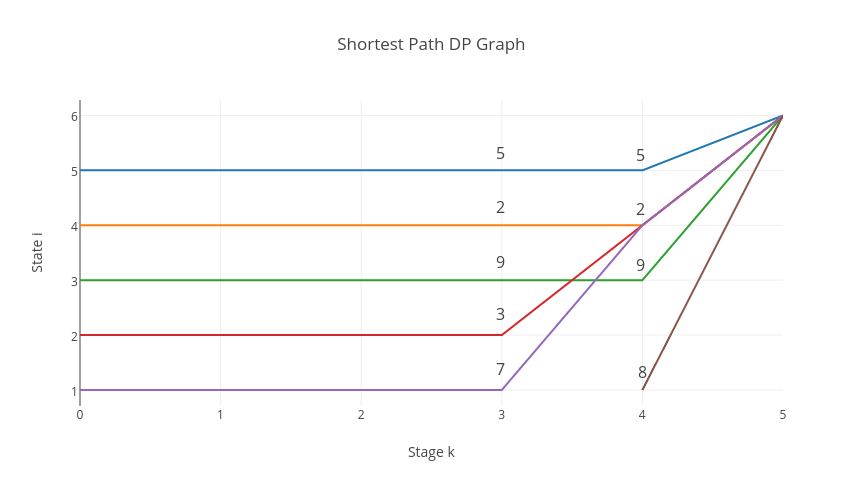
\includegraphics[width=14cm, height=8cm]{Plot2.png} \\
Using the DP algorithm as discussed in class we find the above graph. Hence the shortest path from each node to node 6 is as follows: \\
From node 1: 7 \\
From node 2: 3 \\
From node 3: 9 \\
From node 4: 2 \\
From node 5: 5


%%%%%%%%
% Problem 2 %
%%%%%%%%
\section{Shortest Path via Label Correcting Methods}

%%%%%%%%
% Problem 3 %
%%%%%%%%
\section{Clustering}


%%%%%%%%
% Problem 4 %
%%%%%%%%
\section{Path Bottleneck Problem}

%%%%%%%%
% Problem 5 %
%%%%%%%%
\section{TSP Computational Assignment}

\end{document}  















